\begin{figure}
    \centering
    \begin{subfigure}[c]{1.0\textwidth}
        \centering
        % img_S3HT-64P3-2GW
        % 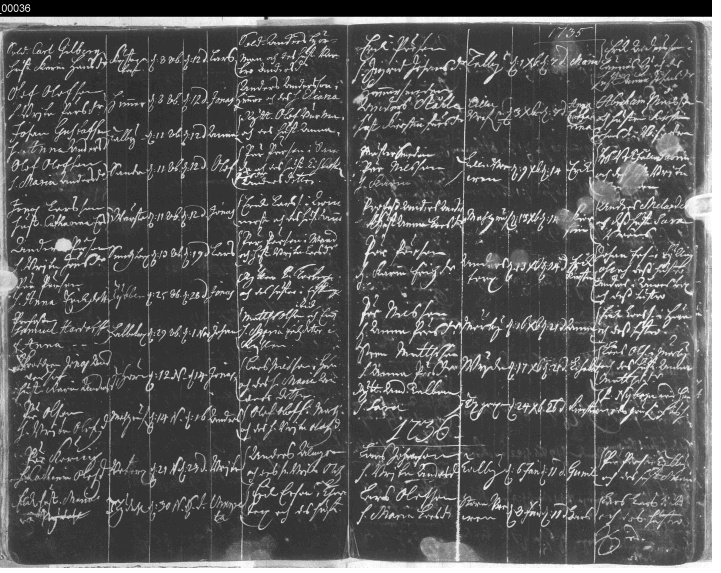
\includegraphics[scale=1.0]{resources/Edited/Orig_processed/img_S3HT-64P3-2GW.jpg}
        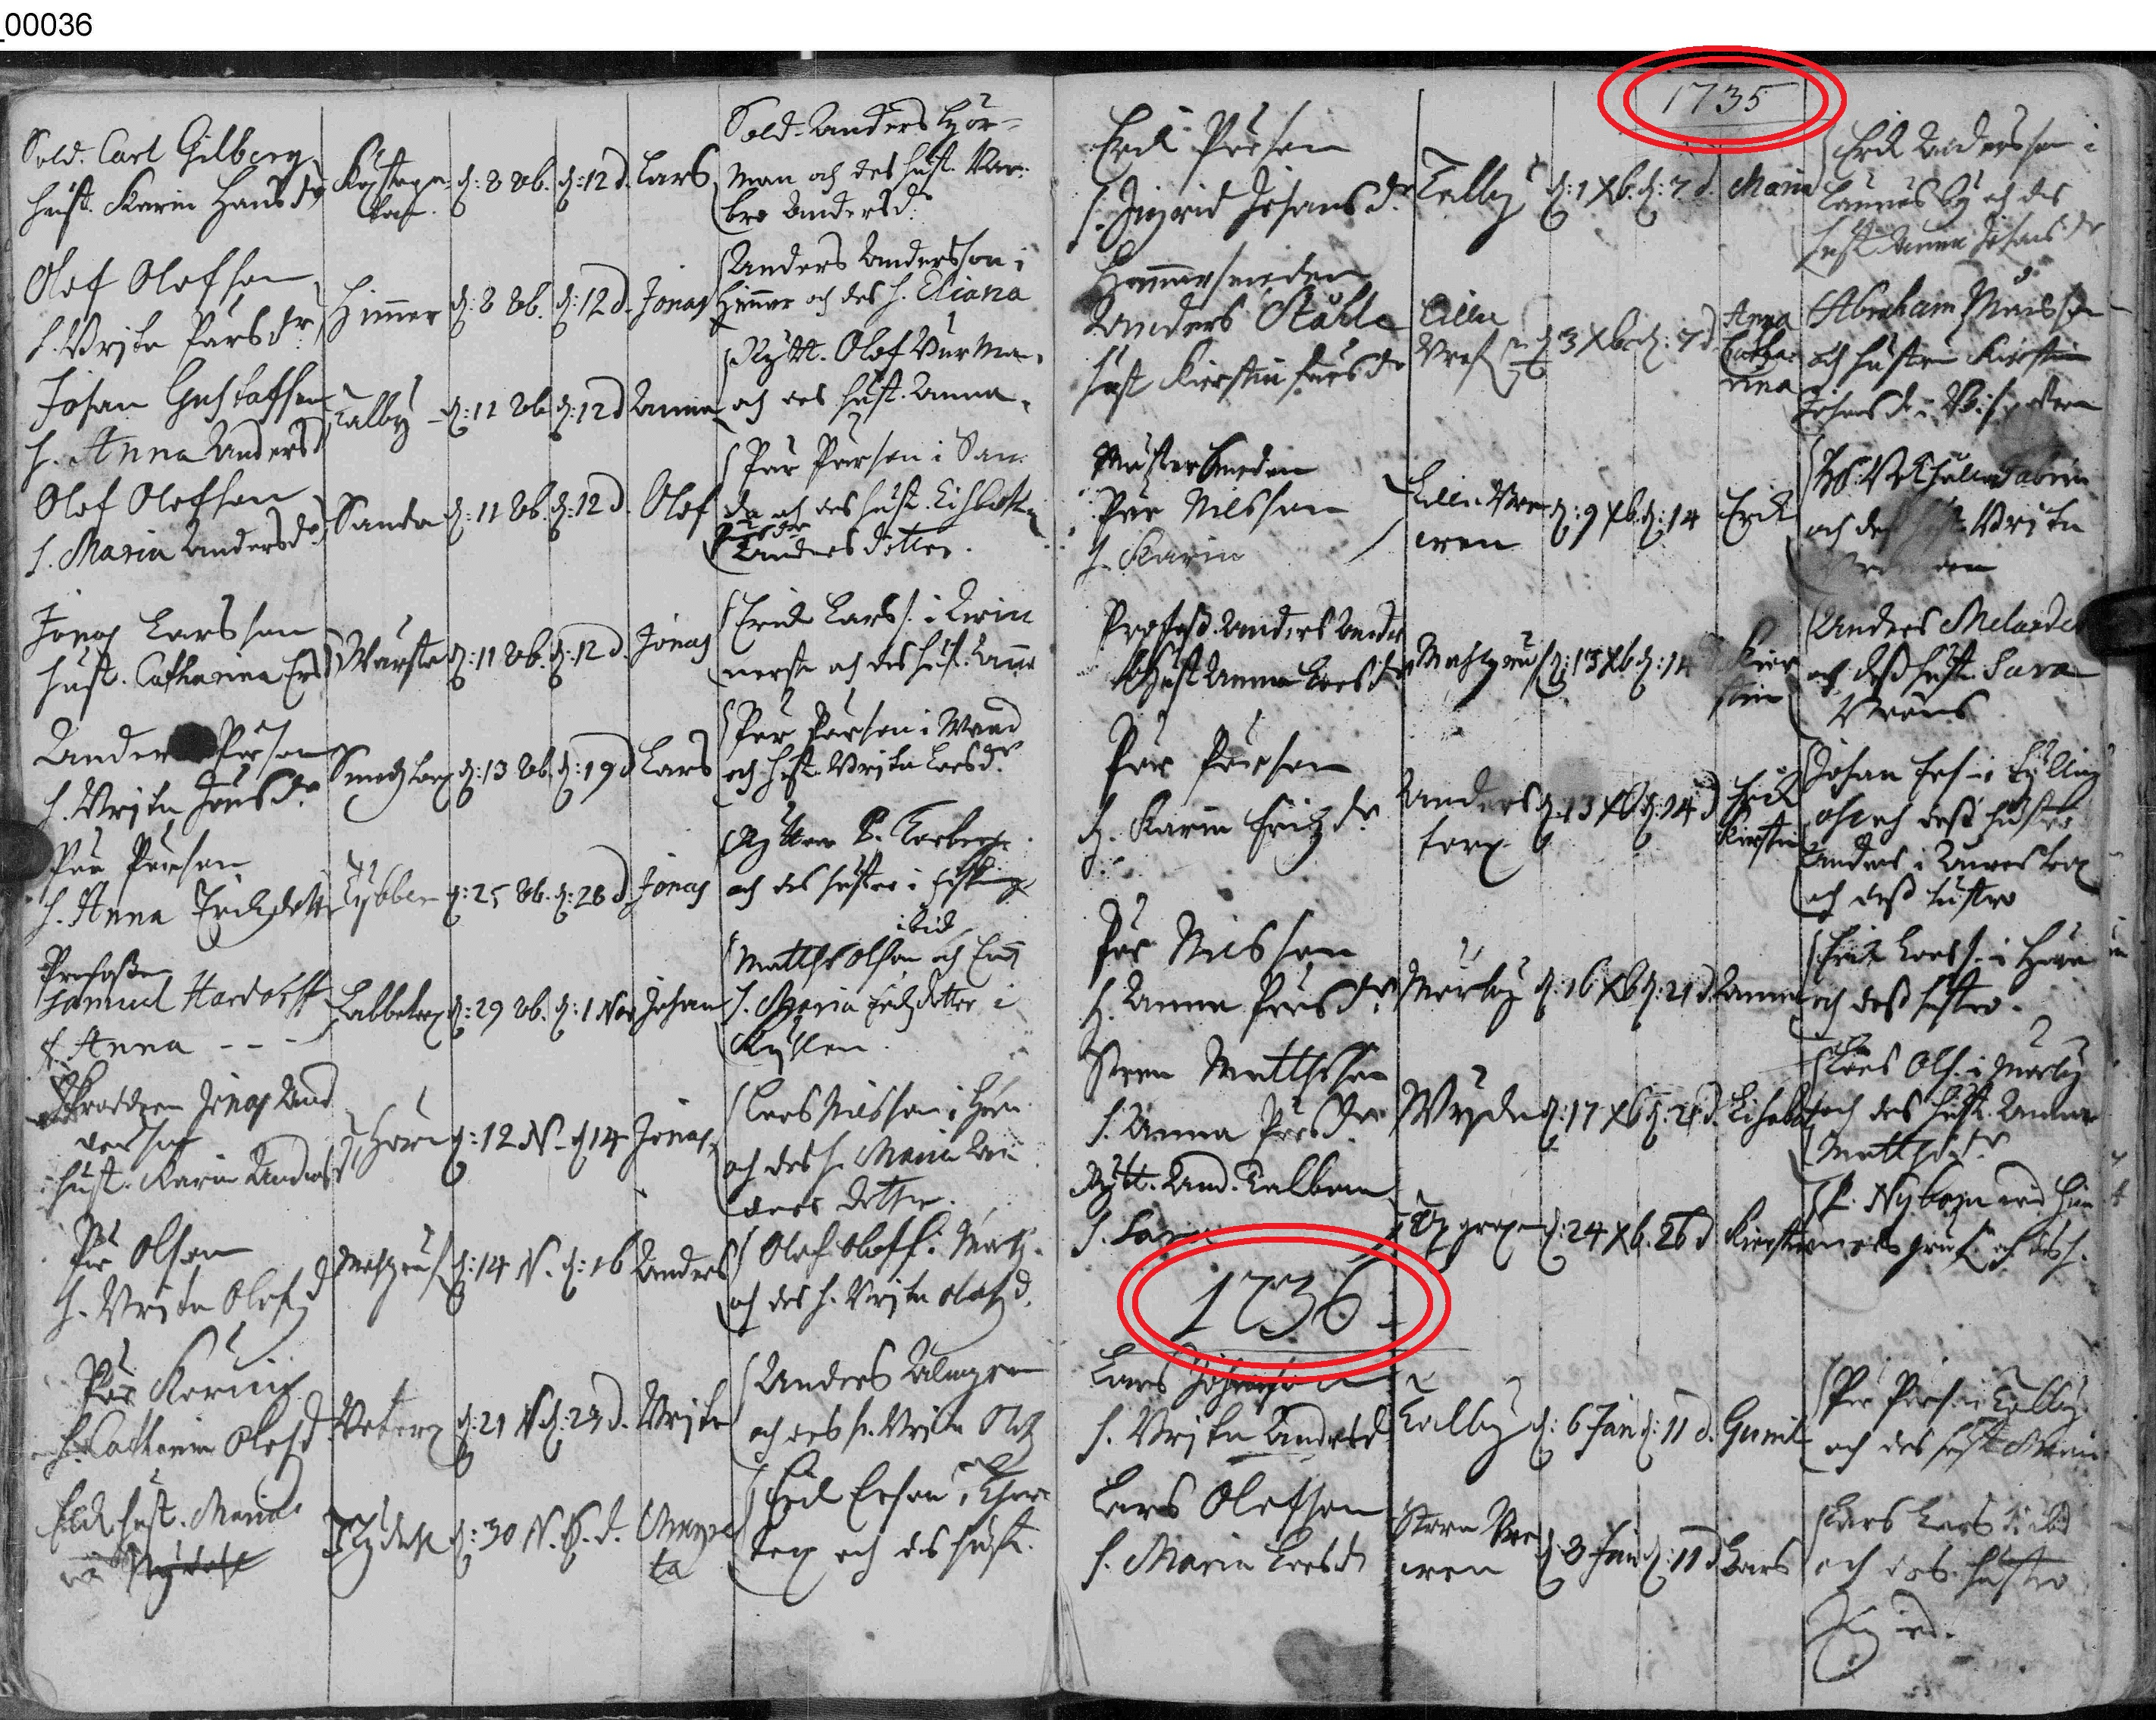
\includegraphics[scale=0.5]{resources/Edited/emph_S3HT-64P3-2GW.jpg}
        \caption{Years are emphasized with double ovals.}
        % \label{fig:jump_prob}
    \end{subfigure}
    \begin{subfigure}[c]{1.0\textwidth}
        \centering
        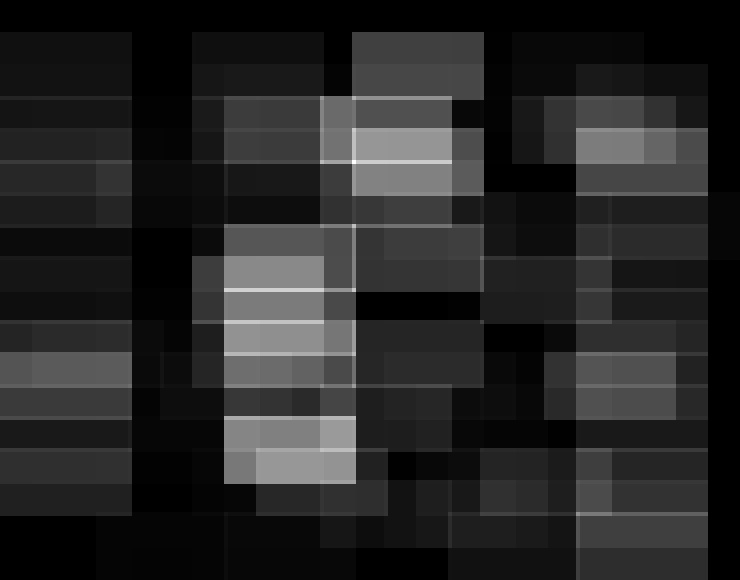
\includegraphics[scale=2.0]{resources/Edited/Orig_att/att_S3HT-64P3-2GW.jpg}
        \caption{The attention focuses on the handwriting and not the years.}
        % \label{fig:jump_log_counts}
    \end{subfigure}
    \caption{Example of a test image that is classified correctly as 1736, even when the two handwritten years are removed from the image. The page comes from the book Asker C:2 in the Örebro collection.}
    \label{fig:edited}
\end{figure}